\section{Load System}
The purpose of this block is to measure the electrical current generated by the Generator and to control the amount of power delivered to a load.

\subsection{Design}
Text

\begin{figure}[H]
	\centering
	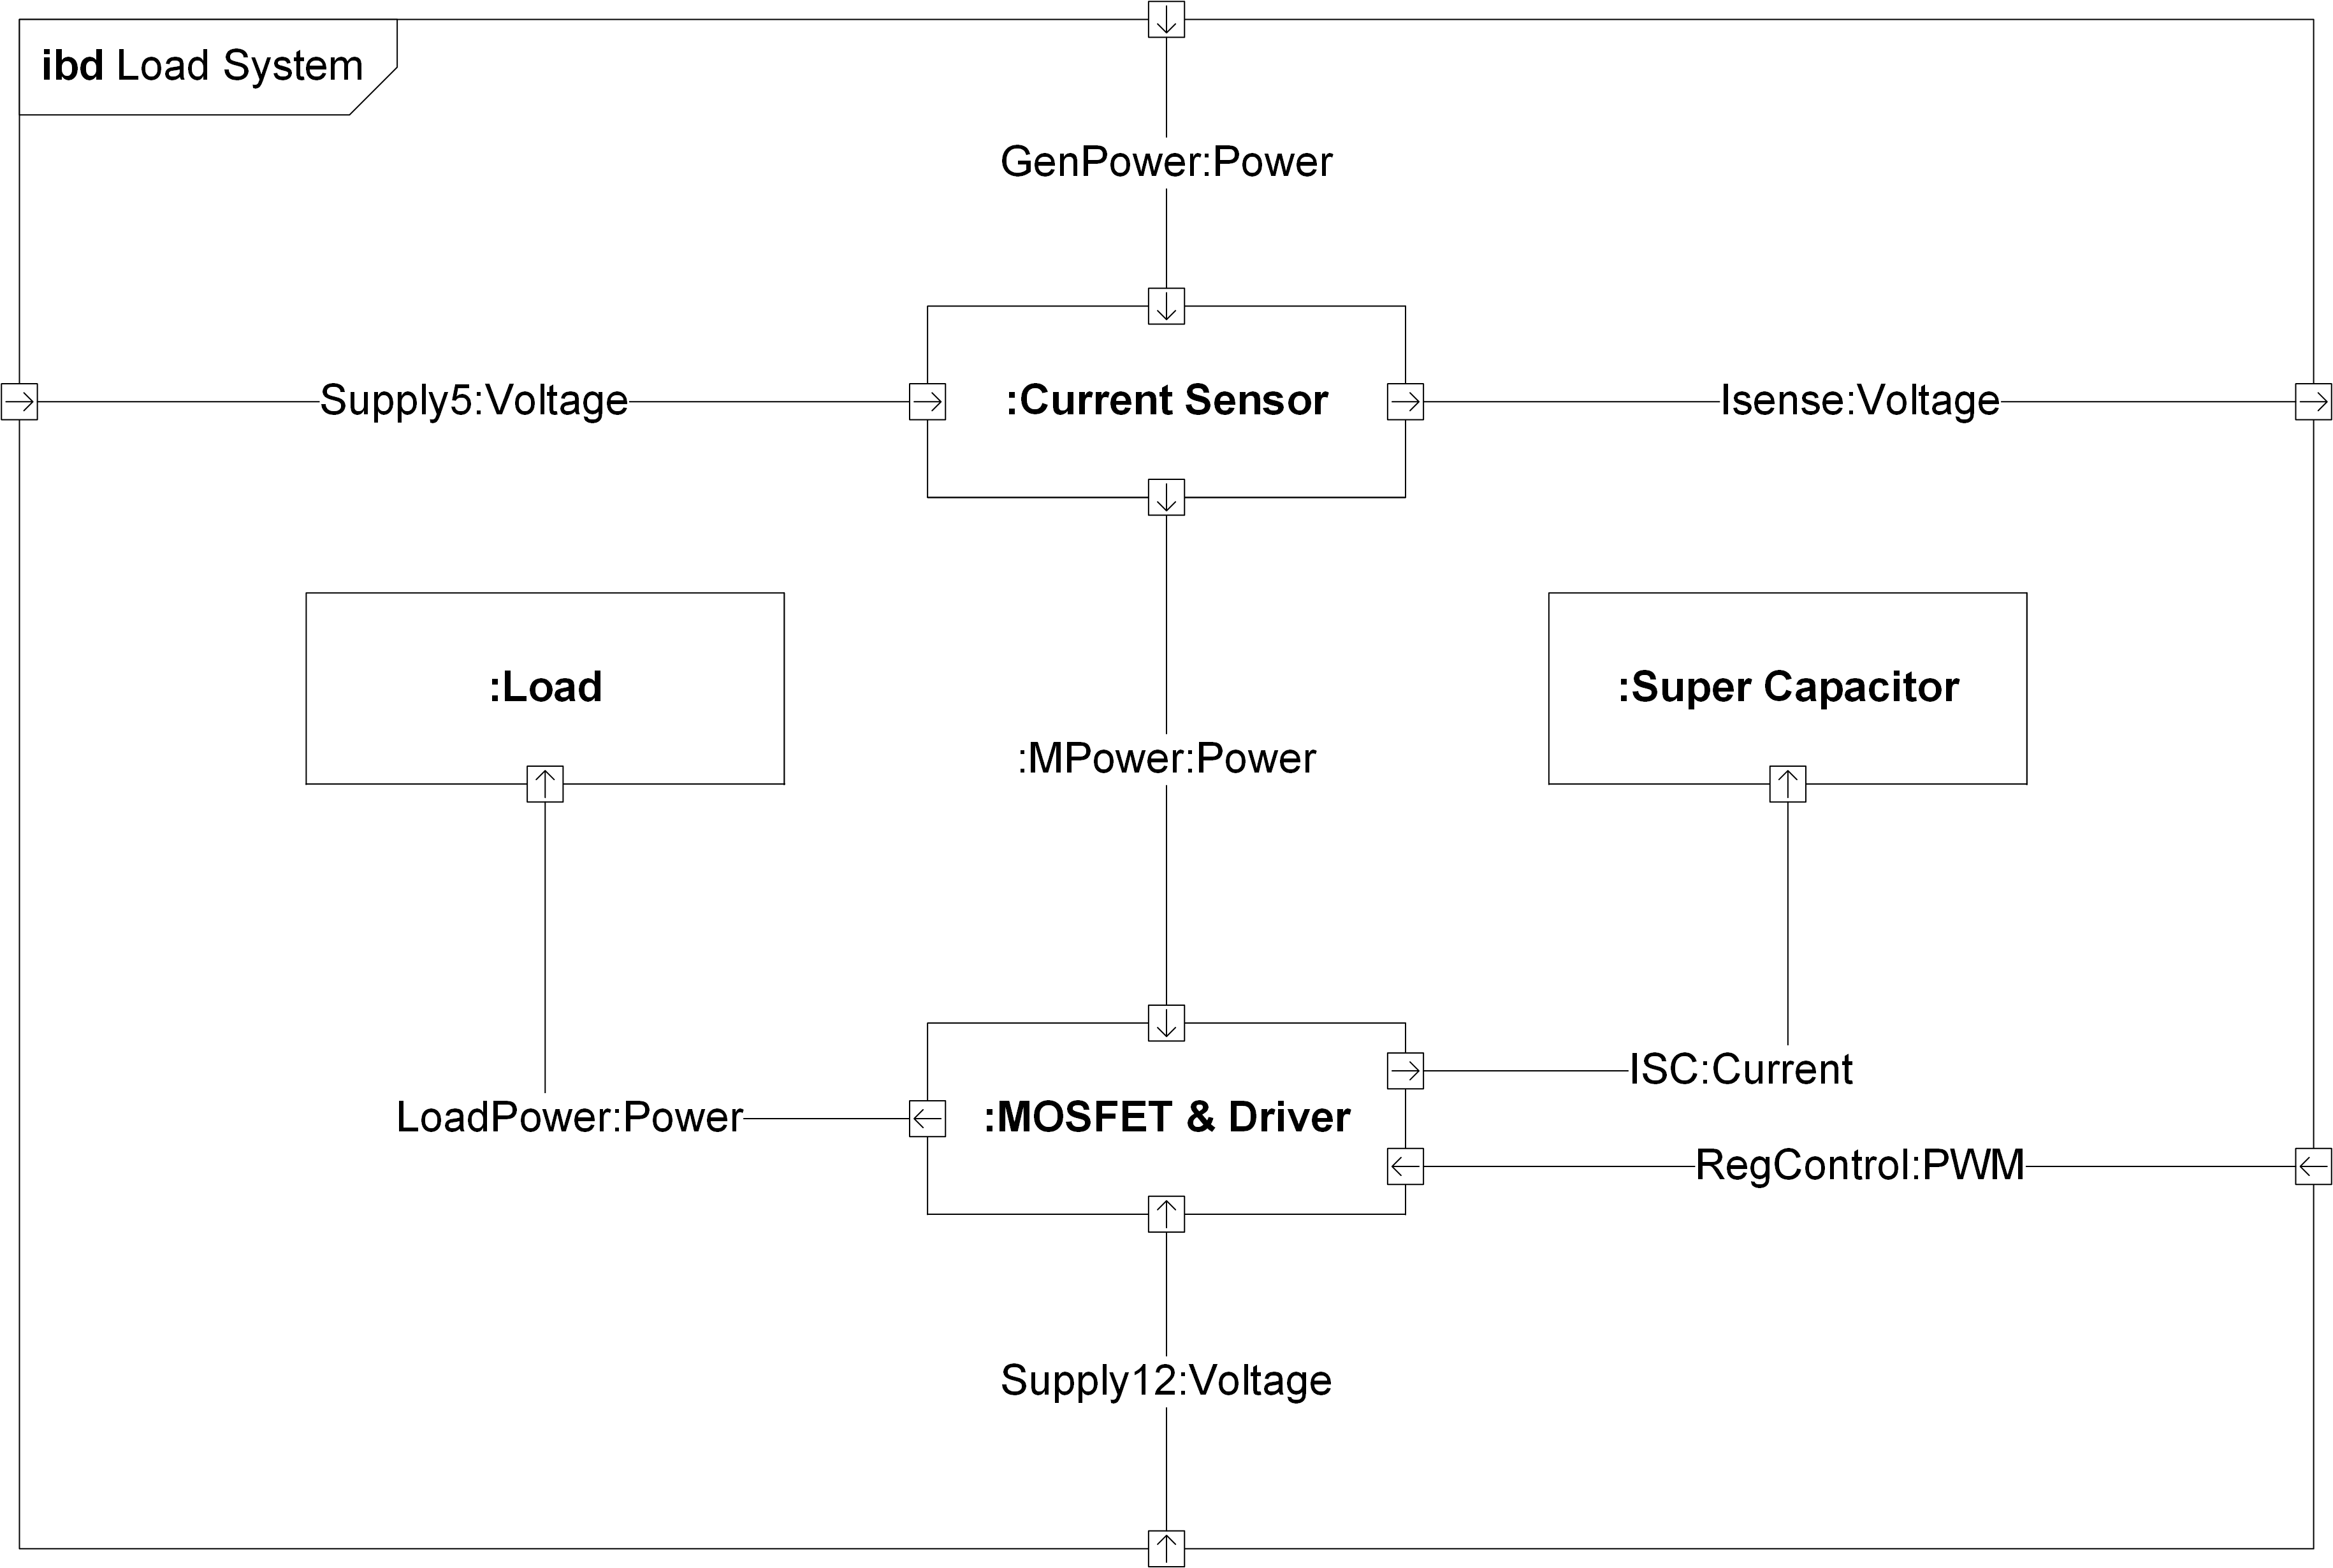
\includegraphics[width=0.7\linewidth]{Hardware/Pictures/IBD_LoadSystem}
	\caption{IBD of the Load System}
	\label{fig:IBD_Load_System}
\end{figure}

Text

\textbf{Current Sensor}\\
Text

\textbf{MOSFET}\\
Text

\textbf{Load}\\
The load serves no other function than converting electrical power into heat.

\subsection{Implementation}
Text

\begin{figure}[H]
	\centering
	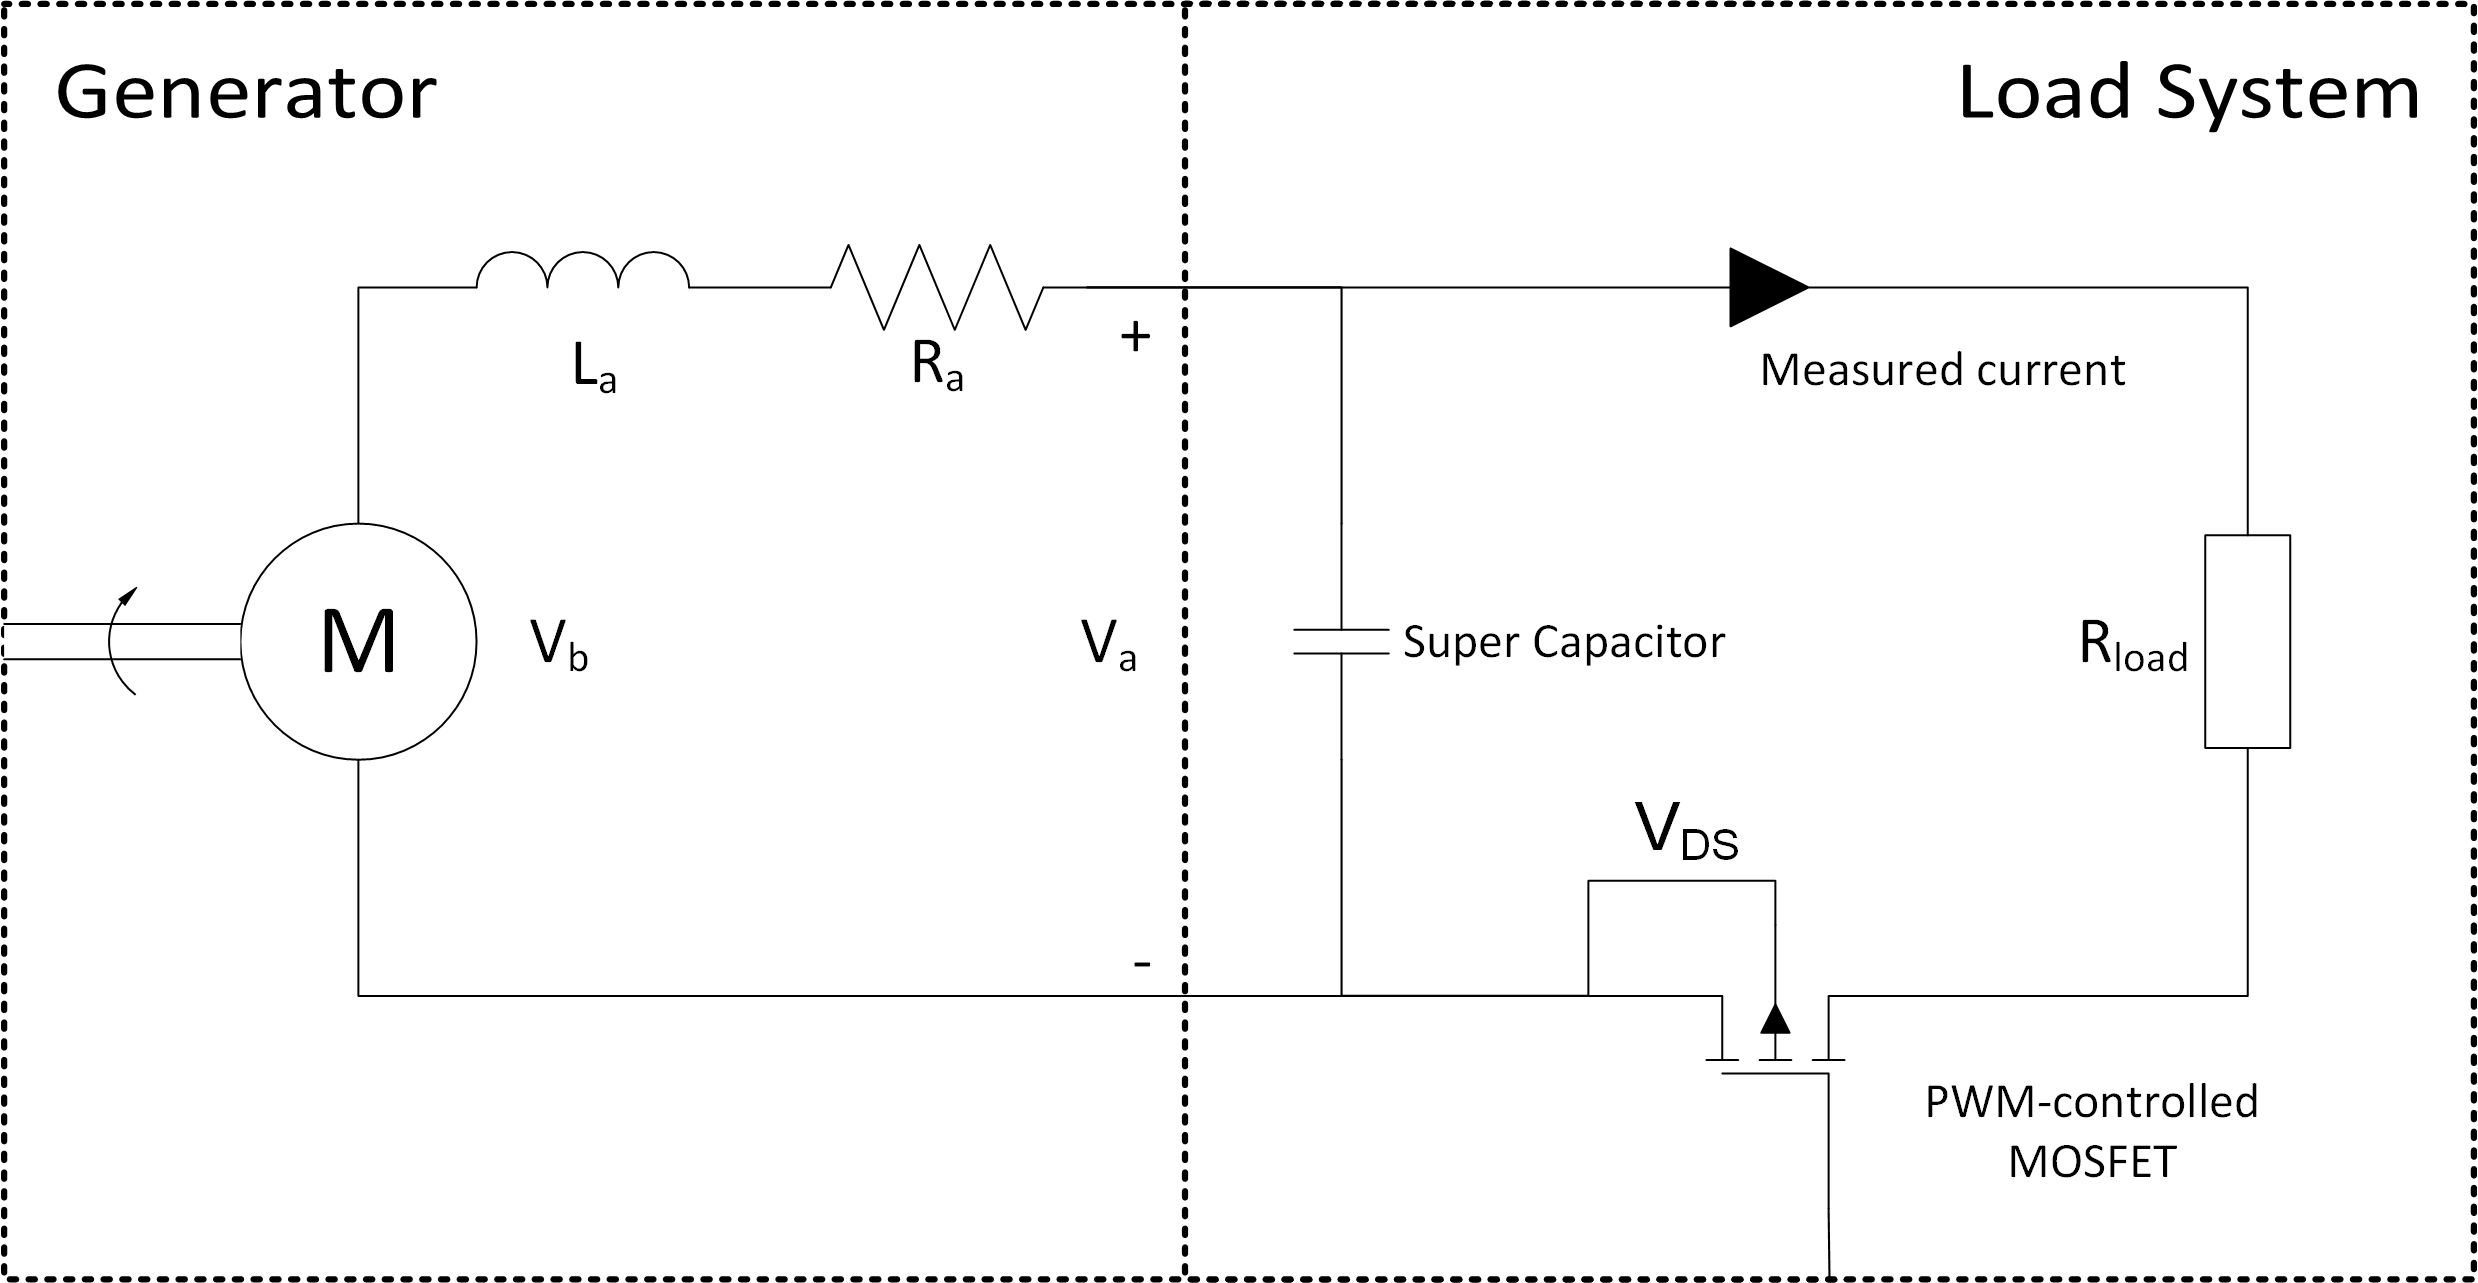
\includegraphics[width=0.7\linewidth]{Hardware/Pictures/LoadSystem}
	\caption{Connection between Generator and Load System}
	\label{fig:Load_System}
\end{figure}

\textbf{Current Sensor}

\textbf{MOSFET}

\textbf{Load}

\subsection{Unity test}
Text